\documentclass[student,noshadow]{ITRslides}
\usepackage{multimedia}

\usepackage[absolute,overlay]{textpos}
\renewcommand{\vec}[1]{\boldsymbol{#1}}
\addbibresource{ref.bib}
\graphicspath{{pics/}{logos/}}
\usepackage{psfrag}
\usepackage[percent]{overpic}
\usepackage{subcaption}
\usepackage{units}
\usepackage{tikz}
\usepackage{pgfplots}
\usepackage{booktabs}
\usetikzlibrary{positioning,shapes,fadings,decorations.pathmorphing,arrows}
\title{Object exploration using haptic information by a human-robot team}
\presenter{Florian Wirnshofer, Benedikt Schmidt}

\supervisor{Denis Cehajic}
\typeofpres{Project Laboratory Cognitive Robotics and Control}

\definecolor{light-gray}{gray}{0.95}

\newcommand*\MyBlue{%
  \item[\color{blue}\scalebox{0.9}{\textbullet}]}
\newcommand*\MyRed{%
  \item[\color{red}\scalebox{0.9}{\textbullet}]}
%\nocite{*}

\renewcommand{\vec}[1]{\boldsymbol{#1}} 
% Alle indizes in Normalschrift ausser Läuferindizes
\newcommand{\scr}[1]{\mathrm{#1}} 

%%%%%%%%%%%%%%%%%%%%%%%%%%%%%%%%%%%%%%%%%%%%%%%%%%%%%%%%%%%%%%%%%%%%%%%%%%%%%%%%

\begin{document}

\begin{frame}
	\titlepage
\end{frame}

%%%%%%%%%%%%%%%%%%%%%%%%%%%%%%%%%%%%%%%%%%%%%%%%%%%%%%%%%%%%%%%%%%%%%%%%%%%%%%%%
%INTRODUCTION , MOTIVATION
%%%%%%%%%%%%%%%%%%%%%%%%%%%%%%%%%%%%%%%%%%%%%%%%%%%%%%%%%%%%%%%%%%%%%%%%%%%%%%%%
\begin{frame}
	\frametitle{Content}
	\tableofcontents
\end{frame}

\section{Online Load Estimation}
\begin{frame}
	\frametitle{Motivation}
\end{frame}

\begin{frame}
	\frametitle{Task}
	\begin{block}{Goal}
		Human-Robot cooperative estimation of load uncertainties.
	\end{block}
	\vspace{2mm}
	\begin{block}{Key-Questions}
		\begin{itemize}
			\item How to fuse and process sensor feedback, resulting in a reliable load-identification?
			\item How should the agents excite the load?
			\item How to exchange information between agents?
		\end{itemize}	   
	\end{block}	
\end{frame}

\begin{frame}
	\frametitle{Online Load Estimation}
	
	\begin{columns}
		\centering
		\begin{column}{0.25\textwidth}
			\begin{figure}
				\centering
				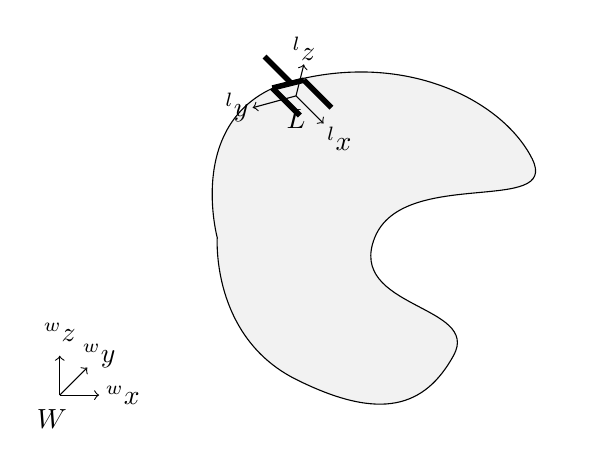
\begin{tikzpicture}
	% world frame
	\draw[arrows=->,line width=0.4pt] (0, 0) -- (0.5, 0);
	\draw[arrows=->,line width=0.4pt] (0, 0) -- (0.35, 0.35);
	\draw[arrows=->,line width=0.4pt] (0, 0) -- (0, 0.5);
	\node at (0.8, 0) {$^wx$};
	\node at (0.5, 0.5) {$^wy$};
	\node at (0, 0.8) {$^wz$};
	\node at (-0.1, -0.3) {$W$};
	
	% load
	\draw[fill,light-gray,draw=black] plot[smooth, tension=1.3] coordinates {(2, 2) (3, 4) (6, 3) (4, 2) (5, 0.5) (3, 0.2) (2, 2)};
	
	% load frame
	\draw[arrows=->,line width=0.4pt] (3, 3.8) -- (3.35, 3.45);
	\draw[arrows=->,line width=0.4pt] (3, 3.8) -- (2.45, 3.65);
	\draw[arrows=->,line width=0.4pt] (3, 3.8) -- (3.1, 4.2);
	\node at (3.55, 3.25) {$^lx$};
	\node at (2.25, 3.65) {$^ly$};
	\node at (3.1, 4.4) {$^lz$};
	\node at (3, 3.5) {$L$};
	
	% gripper
	\draw[draw=black,line width=2pt] (3.1, 4) -- (3.45, 3.65);
	\draw[draw=black,line width=2pt] (2.7, 3.9) -- (3.05, 3.55);
	\draw[draw=black,line width=2pt] (3.1, 4) -- (2.7, 3.9);
	\draw[draw=black,line width=2pt] (2.6, 4.3) -- (2.95, 3.95);
\end{tikzpicture} 
			\end{figure}
		\end{column}
				 		
		\begin{column}{0.75\textwidth}
			Model:\\ \cite{literaturstelle2}\\
			%\vspace{0.1cm}
			\[^\scr{L}\vec{F} = m {^\scr{W}}\vec{\ddot{p}} + m ^\scr{L}\vec{g} + ^\scr{L}\vec{\dot{\omega}} \times m ^\scr{L}\vec{c} + ^\scr{L}\vec{\omega} \times (^\scr{L}\vec{\omega} \times m ^\scr{L}\vec{c})\]
			\[^\scr{L}\vec{N} = ^\scr{L}\vec{I} ^\scr{L}\vec{\dot{\omega}} + ^\scr{L}\vec{\omega} \times (^\scr{L}\vec{I} ^\scr{L}\vec{\omega}) + m ^\scr{L}\vec{c} \times {^\scr{W}}\vec{\ddot{p}} + m ^\scr{L}\vec{c} \times ^\scr{L}\vec{g}\]
						
			\vspace{0.1cm}
			$\vec{\ddot{p}}$ EEF acceleration\\
			$m$ Object mass\\
			$\vec{I}$  Object inertia tensor
		\end{column}
	\end{columns}
	\vspace{0.2cm}
	RLS Estimation-Parameters: \\
	$\vec{\Theta} = [m, m c_\scr{x}, m c_\scr{y}, m c_\scr{z}, I_\scr{xx}, I_\scr{xy}, I_\scr{xz}, I_\scr{yy},I_\scr{yz}, I_\scr{zz}]^\scr{T}$ \\
\end{frame}

\begin{frame}
	\frametitle{Cooperative Online Load Estimation}
	\begin{columns}
		\begin{column}{0.5\textwidth}
			\begin{figure}
				\centering
				\resizebox{4cm}{!}{
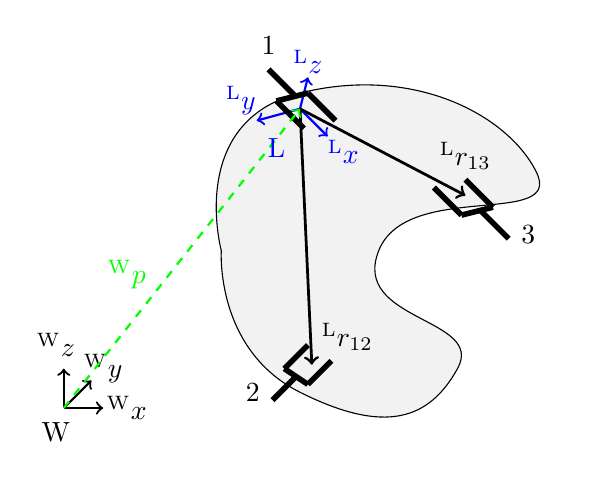
\begin{tikzpicture}
	% world frame
	\draw[arrows=->,line width=0.8pt] (0, 0) -- (0.5, 0);
	\draw[arrows=->,line width=0.8pt] (0, 0) -- (0.35, 0.35);
	\draw[arrows=->,line width=0.8pt] (0, 0) -- (0, 0.5);
	\node at (0.8, 0) {{$^\mathrm{W}x$}};
	\node at (0.5, 0.5) {{$^\mathrm{W}y$}};
	\node at (-0.1, 0.8) {{$^\mathrm{W}z$}};
	\node at (-0.1, -0.3) {W};	
	% load
	\draw[fill,light-gray,draw=black] plot[smooth, tension=1.3] coordinates {(2, 2) (3, 4) (6, 3) (4, 2) (5, 0.5) (3, 0.2) (2, 2)};
	
	% load frame
	\draw[draw=blue,arrows=->,line width=0.8pt] (3, 3.8) -- (3.35, 3.45);
	\draw[draw=blue,arrows=->,line width=0.8pt] (3, 3.8) -- (2.45, 3.65);
	\draw[draw=blue,arrows=->,line width=0.8pt] (3, 3.8) -- (3.1, 4.2);
	\node[text=blue] at (3.55, 3.25) {{$^\mathrm{L}x$}};
	\node[text=blue] at (2.25, 3.9) {{$^\mathrm{L}y$}};
	\node[text=blue] at (3.1, 4.4) {{$^\mathrm{L}z$}};
	
		
	
	
	% gripper one
	\draw[draw=black,line width=2pt] (3.1, 4) -- (3.45, 3.65);
	\draw[draw=black,line width=2pt] (2.7, 3.9) -- (3.05, 3.55);
	\draw[draw=black,line width=2pt] (3.1, 4) -- (2.7, 3.9);
	\draw[draw=black,line width=2pt] (2.6, 4.3) -- (2.95, 3.95);
	\node at (2.6, 4.6) {$1$};
	
	% gripper two
	\draw[draw=black,line width=2pt] (2.8, 0.5) -- (3.1, 0.3);
	\draw[draw=black,line width=2pt] (2.8, 0.5) -- (3.1, 0.8);
	\draw[draw=black,line width=2pt] (3.1, 0.3) -- (3.4, 0.6);
	\draw[draw=black,line width=2pt] (2.65, 0.1) -- (2.95, 0.4);
	\node at (2.4, 0.2) {$2$};
	
	% gripper three
	\draw[draw=black,line width=2pt] (5.1, 2.9) -- (5.45, 2.55);
	\draw[draw=black,line width=2pt] (4.7, 2.8) -- (5.05, 2.45);
	\draw[draw=black,line width=2pt] (5.45, 2.55) -- (5.05, 2.45);
	\draw[draw=black,line width=2pt] (5.65, 2.15) -- (5.3, 2.5);
	\node at (5.9, 2.2) {$3$};
	
	% grasping offsets
	\draw[arrows=->,line width=1pt] (3, 3.8) -- (3.15, 0.55);
	\node at (3.6, 0.9) {$^\scr{L}\vec{r}_{12}$};
	\draw[arrows=->,line width=1pt] (3, 3.8) -- (5.1, 2.7);
	\node at (5.1, 3.2) {$^\scr{L}\vec{r}_{13}$};
	
	\draw[->,thick,dashed,green](0, 0) -- (3, 3.8);
	\node[text=blue] at (2.7, 3.3) {L};
	\node[text=green] at (0.8, 1.7) {$^\scr{W}\vec{p}$};
\end{tikzpicture}
}
			\end{figure}	
		\end{column}
		\begin{column}{0.5\textwidth}
			$^\scr{L}\vec{F}_i$: Forces acting at grasping point $i$, measured w.r.t. the EEF frame L.\\ \vspace{0.3cm}
			$^\scr{L}\vec{N}_i$: Torques acting at grasping point $i$, measured w.r.t. the EEF frame L.\\
		\end{column}
	\end{columns}
	
	\begin{align*} 
		\sum_{i = 1}^{n}  {^\scr{L}}\vec{F}_{i}                                                                   & =  f\left(^\scr{W}\vec{\ddot{p}},^\scr{L}\vec{\omega},^\scr{L}\vec{\dot{\omega}},^\scr{L}\vec{c},m\right)                          \\ 
		\sum_{i = 1}^n {^\scr{L}}\vec{N}_{i} + \sum_{i = 2}^n {^\scr{L}}\vec{r}_{1i} \times {^\scr{L}}\vec{F}_{i} & = f\left({^\scr{W}}\vec{\ddot{p}},{^\scr{L}}\vec{\omega}{^\scr{L}},\vec{\dot{\omega}},{^\scr{L}}\vec{c},{^\scr{L}}\vec{I},m\right) 
	\end{align*}
\end{frame}

\begin{frame}
	\frametitle{Cooperative Online Load Estimation}
	\begin{columns}
		\begin{column}{0.6\textwidth}
			\begin{overpic}[width=\textwidth]{pics/setup}
				\put(6,0){\color{red}{$x$}}
				\put(10,10){\color{green}{$y$}}
				\put(5,15){\color{blue}{$z$}}
				\put(69,46){\small  $\mathrm{a}^{1}$)}
				\put(55,64){\small  $\mathrm{a}^{2}$)}
				\put(48,47){\small  $\mathrm{a}^{3}$)}
				\put(35,51){\small b)}
				\put(58,48){\tiny \color{red}{CoM}}
			\end{overpic}
		\end{column}
		
		\begin{column}{0.4\textwidth}
			$\mathrm{a}^{1}$): Robot EEF grasping point, \textsc{JR3} F-T Sensor, tracked\\ \vspace{0.3cm}
			$\mathrm{a}^{2}$), $\mathrm{a}^{3}$): Human agent grasping points, \textsc{JR3} F-T Sensor, tracked\\ \vspace{0.3cm}
			b):  Vibrotactile wristband
		\end{column}
	\end{columns}
\end{frame}

\begin{frame}
	\frametitle{Excitation Pattern}
	\simpleblock{
		\begin{small}
			\begin{center}
				RLS convergence prerequisites
			\end{center}
		\end{small}
	}
	\vspace{1cm}	
	\begin{itemize}
		\item Reference trajectory must be persistently exciting(PE)
		\item Non-zero acceleration of EEF in 6-DoF \cite{literaturstelle3}
	\end{itemize}
	\vspace{1cm}
	\textsc{Challenge}: Satisfaction of actuator limits, especially when trying to identify big objects.
\end{frame}

\section{Experimental Results}
\begin{frame}
	\frametitle{Data Acquisition}
	\begin{columns}
		\begin{column}{0.35\textwidth}
			\begin{figure}
				\centering
				\resizebox{4cm}{!}{
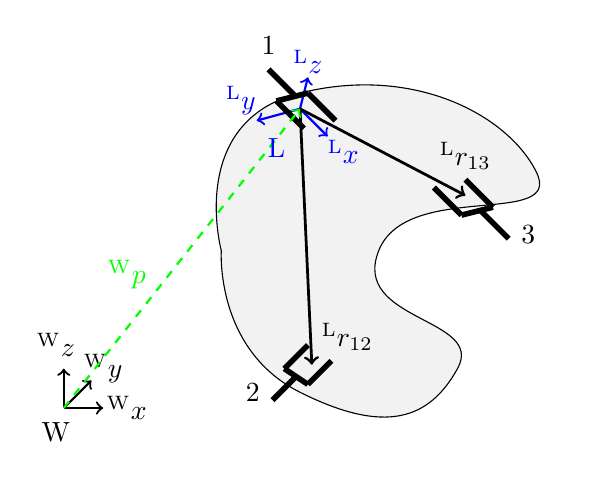
\begin{tikzpicture}
	% world frame
	\draw[arrows=->,line width=0.8pt] (0, 0) -- (0.5, 0);
	\draw[arrows=->,line width=0.8pt] (0, 0) -- (0.35, 0.35);
	\draw[arrows=->,line width=0.8pt] (0, 0) -- (0, 0.5);
	\node at (0.8, 0) {{$^\mathrm{W}x$}};
	\node at (0.5, 0.5) {{$^\mathrm{W}y$}};
	\node at (-0.1, 0.8) {{$^\mathrm{W}z$}};
	\node at (-0.1, -0.3) {W};	
	% load
	\draw[fill,light-gray,draw=black] plot[smooth, tension=1.3] coordinates {(2, 2) (3, 4) (6, 3) (4, 2) (5, 0.5) (3, 0.2) (2, 2)};
	
	% load frame
	\draw[draw=blue,arrows=->,line width=0.8pt] (3, 3.8) -- (3.35, 3.45);
	\draw[draw=blue,arrows=->,line width=0.8pt] (3, 3.8) -- (2.45, 3.65);
	\draw[draw=blue,arrows=->,line width=0.8pt] (3, 3.8) -- (3.1, 4.2);
	\node[text=blue] at (3.55, 3.25) {{$^\mathrm{L}x$}};
	\node[text=blue] at (2.25, 3.9) {{$^\mathrm{L}y$}};
	\node[text=blue] at (3.1, 4.4) {{$^\mathrm{L}z$}};
	
		
	
	
	% gripper one
	\draw[draw=black,line width=2pt] (3.1, 4) -- (3.45, 3.65);
	\draw[draw=black,line width=2pt] (2.7, 3.9) -- (3.05, 3.55);
	\draw[draw=black,line width=2pt] (3.1, 4) -- (2.7, 3.9);
	\draw[draw=black,line width=2pt] (2.6, 4.3) -- (2.95, 3.95);
	\node at (2.6, 4.6) {$1$};
	
	% gripper two
	\draw[draw=black,line width=2pt] (2.8, 0.5) -- (3.1, 0.3);
	\draw[draw=black,line width=2pt] (2.8, 0.5) -- (3.1, 0.8);
	\draw[draw=black,line width=2pt] (3.1, 0.3) -- (3.4, 0.6);
	\draw[draw=black,line width=2pt] (2.65, 0.1) -- (2.95, 0.4);
	\node at (2.4, 0.2) {$2$};
	
	% gripper three
	\draw[draw=black,line width=2pt] (5.1, 2.9) -- (5.45, 2.55);
	\draw[draw=black,line width=2pt] (4.7, 2.8) -- (5.05, 2.45);
	\draw[draw=black,line width=2pt] (5.45, 2.55) -- (5.05, 2.45);
	\draw[draw=black,line width=2pt] (5.65, 2.15) -- (5.3, 2.5);
	\node at (5.9, 2.2) {$3$};
	
	% grasping offsets
	\draw[arrows=->,line width=1pt] (3, 3.8) -- (3.15, 0.55);
	\node at (3.6, 0.9) {$^\scr{L}\vec{r}_{12}$};
	\draw[arrows=->,line width=1pt] (3, 3.8) -- (5.1, 2.7);
	\node at (5.1, 3.2) {$^\scr{L}\vec{r}_{13}$};
	
	\draw[->,thick,dashed,green](0, 0) -- (3, 3.8);
	\node[text=blue] at (2.7, 3.3) {L};
	\node[text=green] at (0.8, 1.7) {$^\scr{W}\vec{p}$};
\end{tikzpicture}
}
			\end{figure}	
		\end{column}
		\begin{column}{0.65\textwidth}
			\begin{tabular}{llr}
				\toprule
				Information                                   & Tool              & Frame Rate $\left[\mathrm{Hz}\right]$ \\
				\midrule
				${^\scr{L}}\vec{F}_{i},{^\scr{L}}\vec{N}_{i}$ & \textsc{JR3}      & 8000 $\rightarrow$ 100                \\
				                                              & \textsc{Qualisys} & 100                                   \\
				$^\scr{L}\vec{\omega}$                        & \textsc{Qualisys} & 100                                   \\
				$^\scr{W}\vec{p}$                             & \textsc{Qualisys} & 100                                   \\
				$^\scr{L}\vec{r}_{1i}$                        & \textsc{Qualisys} & 100                                   \\
				\bottomrule
			\end{tabular}
		\end{column}
	\end{columns}
	\textsc{Issue}: Noise prone first and second derivatives\\
	\textsc{Solution}: Butterworth lowpass filter (Order: 3, $\omega_\mathrm{CutOff} = 30 \mathrm{Hz}$)
\end{frame}

\begin{frame}
	\frametitle{Experimental Results}
	Conducted experiments:
	\vspace{0.5cm}
	\begin{itemize}
		\item Multiple grasping points in simulation
		\item Multiple grasping points
	\end{itemize}
\end{frame}

\begin{frame}
	%Benedikt
	\frametitle{Simulation Results with Noise ($P = \unit[0.05]{W}$)}
	\begin{center}
		\begin{figure}
			\psfrag{x}[tr][br]{$t\left[\mathrm{s}\right]$}
			\psfrag{y1}[br][tr]{$\epsilon_\scr{Mass}$}
			\psfrag{y2}[br][tr]{$\epsilon_\scr{CoM}$}
			\psfrag{one}[c][Bc]{$0$}
			\psfrag{two}[c][Bc]{$1$}
			\psfrag{thr}[c][Bc]{$2$}
			\psfrag{fou}[c][Bc]{$3$}
			\psfrag{fiv}[c][Bc]{$4$}
			\psfrag{six}[c][Bc]{$5$}
			\psfrag{lllllllll}[Br][Br]{$10^{-6}$}
			\psfrag{lllllllli}[Br][Br]{$10^{-4}$}
			\psfrag{lllllllil}[Br][Br]{$10^{-2}$}
			\psfrag{lllllllii}[Br][Br]{$10^0$}
			\psfrag{llllllill}[Br][Br]{$10^{-10}$}
			\psfrag{llllllili}[Br][Br]{$10^{-5}$}
			\psfrag{lllllliil}[Br][Br]{$10^0$}
			\psfrag{cerror1}[][]{\tiny  $c_{x}$}
			\psfrag{cerror2}[][]{\tiny $c_{y}$}
			\psfrag{cerror3}[][]{\tiny $c_{z}$}
			\begin{overpic}[width=0.8\textwidth]{fig/mass_multi_noise.eps}
			\put(-3,50){\rotatebox{90}{$\epsilon_m \left[\mathrm{kg}\right]$}}
			\put(-3,15){\rotatebox{90}{$\epsilon_{\vec{c}} \left[\mathrm{m}\right]$}}
			\end{overpic}
		\end{figure}
		\vspace{0.3cm}
		Mass $m$ and CoM $\vec{c}$ with multiple grasping points in simulation
	\end{center}
\end{frame}

\begin{frame}
	%Benedikt
	\frametitle{Simulation Results with Noise ($P = \unit[0.05]{W}$)}
	\begin{center}
		\centering
		\begin{figure}
			\psfrag{xaxis}[tr][br]{$t\left[\mathrm{s}\right]$}
			\psfrag{yaxis}[br][tr]{$\epsilon_{\scr{Inertia}}$}
			\psfrag{one}[c][Bc]{$0$}
			\psfrag{two}[c][Bc]{$1$}
			\psfrag{thr}[c][Bc]{$2$}
			\psfrag{fou}[c][Bc]{$3$}
			\psfrag{fiv}[c][Bc]{$4$}
			\psfrag{six}[c][Bc]{$5$}
			\psfrag{lllllllll}[Br][Br]{$10^{-10}$}
			\psfrag{lllllllli}[Br][Br]{$10^{-6}$}
			\psfrag{lllllllil}[Br][Br]{$10^{-2}$}
			\psfrag{lllllllii}[Br][Br]{$10^2$}
			\psfrag{Ierror1}[][]{\tiny \  $I_{xx}$}
			\psfrag{Ierror2}[][]{\tiny \  $I_{yy}$}
			\psfrag{Ierror3}[][]{\tiny \  $I_{zz}$}
			\psfrag{Ierror4}[][]{\tiny \  $I_{xy}$}
			\psfrag{Ierror5}[][]{\tiny \  $I_{xz}$}
			\psfrag{Ierror6}[][]{\tiny \  $I_{yz}$}
			\begin{overpic}[width=0.8\textwidth]{fig/inertia_multi_noise.eps}
				\put(-3,20){\rotatebox{90}{$\epsilon_{\vec{I}} \left[\mathrm{kg} \, \mathrm{m}^2\right]$}}
			\end{overpic}
		\end{figure}
		\vspace{0.5cm}
		Inertia tensor error with multiple grasping points in simulation
	\end{center}
\end{frame}

\begin{frame}
	\frametitle{Multiple Grasping Points}
	\begin{center}
		\begin{figure}
			\centering	
			\psfrag{xaxis}[tr][br]{$t\left[\mathrm{s}\right]$}
			\psfrag{yaxis}[bc][tr]{$I\left[\scr{kg}/\scr{m}^2\right]$}
			\psfrag{one}[c][Br]{$0$}
			\psfrag{two}[c][Br]{$5$}
			\psfrag{thr}[c][Br]{$10$}
			\psfrag{fou}[c][Br]{$15$}
			\psfrag{fiv}[c][Br]{$20$}
			\psfrag{six}[c][Br]{$25$}
			\psfrag{lllllllll}[Br][Br]{$-0.1$}
			\psfrag{lllllllli}[Br][Br]{$-0.05$}
			\psfrag{lllllllil}[Br][Br]{$0$}
			\psfrag{lllllllii}[Br][Br]{$0.05$}
			\psfrag{llllllill}[Br][Br]{$0.1$}
			\psfrag{aaaa}[][]{}
			\begin{overpic}[width=0.8\textwidth]{fig/multiple_grasping_points_human_inertias.eps}
				\put(92,49){\tiny $I_{xx}$}
				\put(92,46){\tiny $I_{yy}$}
				\put(92,43){\tiny $I_{zz}$}
				\put(92,40){\tiny $I_{xy}$}
				\put(92,37){\tiny $I_{xz}$}
				\put(92,34.3){\tiny $I_{yz}$}	
			\end{overpic}
		\end{figure}
		\vspace{0.2cm}
		Inertia Tensor $\vec{I}_\scr{p}$ with multiple grasping points
	\end{center}
\end{frame}

\begin{frame}
	\frametitle{Multiple Grasping Points}
	\begin{center}
		\begin{figure}
			\centering	
			\psfrag{xaxis}[tr][br]{$t\left[\mathrm{s}\right]$}
			\psfrag{yaxism}[bc][tr]{$m\left[\mathrm{kg}\right]$}
			\psfrag{yaxisc}[bc][tr]{$\mathrm{CoM}\left[\mathrm{m}\right]$}
			\psfrag{one}[c][Br]{$0$}
			\psfrag{two}[c][Br]{$5$}
			\psfrag{thr}[c][Br]{$10$}
			\psfrag{fou}[c][Br]{$15$}
			\psfrag{fiv}[c][Br]{$20$}
			\psfrag{six}[c][Br]{$25$}
			\psfrag{lllllllll}[Br][Br]{$3\  $}
			\psfrag{lllllllli}[Br][Br]{$4\ $}
			\psfrag{lllllllil}[Br][Br]{$5\  $}
			\psfrag{lllllllii}[Br][Br]{$6\  $}
			\psfrag{illllllll}[Br][Br]{$-0.4$}
			\psfrag{illllllli}[Br][Br]{$-0.2$}
			\psfrag{illllllil}[Br][Br]{$0$}
			\psfrag{illllllii}[Br][Br]{$0.2$}
			\psfrag{illlllill}[Br][Br]{$0.4$}
			\psfrag{cx}[][]{\tiny $c_x$}
			\psfrag{cy}[][]{\tiny $c_y$}
			\psfrag{cz}[][]{\tiny $c_z$}
			\psfrag{m}[][]{\tiny $m$}
			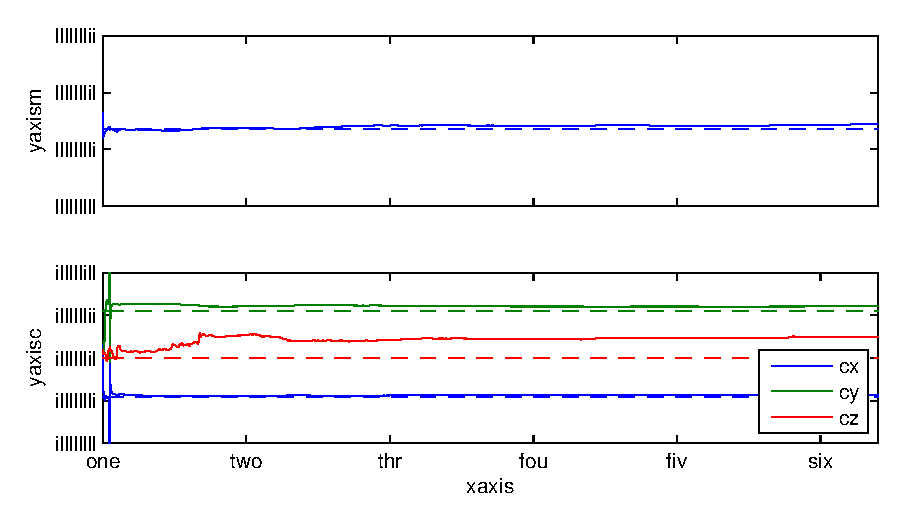
\includegraphics[width=0.8\textwidth]{fig/multiple_grasping_points_human_mass_and_cog.eps}
		\end{figure}
		\vspace{0.2cm}
		Mass $m$ and center of mass $\vec{c}$ with multiple grasping points (dashed lines are the correct values)
	\end{center}
\end{frame}

\begin{frame}
	\frametitle{Summary}
	\begin{block}{Problems}
		\begin{itemize}
			\item Actuator limits
			\item Gripper of robot
			\item Singularity in Euler angles from \textsc{Qualisys}
		\end{itemize}	   
	\end{block}	
	\begin{block}{Possible Solutions}
		\begin{itemize}
			\item Tighter grasp of the robot
			\item Acquisition of quaternions from \textsc{Qualisys}
		\end{itemize}  
	\end{block}	
	\begin{block}{Cooperative Online Load Estimation}
		\begin{itemize}
			\item Estimation of more and heavier objects
			\item Unexperienced human agent needs guidance
		\end{itemize}
	\end{block}	
\end{frame}

\appendix
\begin{frame}
	\frametitle{References}
	\printbibliography
\end{frame}

\end{document}